\documentclass[a4paper]{article}
\usepackage{amsmath}
\usepackage{graphicx}
\usepackage{multicol}
\usepackage{tocloft}

\usepackage{geometry}
 \geometry{
 a4paper,
 total={170mm,257mm},
 left=20mm,
 top=10mm,
 bottom=30mm
 }

\begin{document}

\title{EPFL Machine Learning - Project 1}
\author{
  Pierre-Alexandre Lee, Thomas Garcia, Yves Lamonato\\
  \textit{EPFL Lausanne, Switzerland}
}
\date{\vspace{-5ex}}

\maketitle
\mbox{}\\

\begin{multicols*}{2}

\section{Introduction}
This is the report for the Machine learning EPFL course first project. Using a CERN dataset on the Higgs Boson, we need to find the best model to distinguish background noise from an actual event using machine learning. 

\section{The dataset}
\subsection{Raw data}
We were given the data in two csv files: a training set and a testing set. In both sets we are given a list of measures \textit{xn} with 30 features each. For the training set, the true binary classification is already given to us, \{-1\} for background, \{1\} for true event.
\subsection{Data pre-processing}
\begin{enumerate}
\item \textit{Exploring data}: From the dataset documentation on Kaggle, we know that any missing data was assigned the value \{-999\}. After some exploratory data analysis, we found that those missing data were determined by the \textit{jet} feature. Therefore for each \textit{jet} value we found which feature could be dropped, and made a different model for each \textit{jet} (that is jets \{0\}, \{1\}, and together \{2,3\} since they missed the same features).

\item \textit{Missing values}: After this jet separation, any value left with \{-999\} is replaced with \{0\}.

\item \textit{Data Normalization}: For each \textit{jet} value, we standardize the data by subtracting the mean and dividing by the variance. This helps reducing the range of the variable and thus helps preventing overflow.

\item \textit{Features augmentation}: Finally, in order to increase the family of functions we can find, we added for each column the \textit{sin} and \textit{cos} of the column, and for each column that only has positive elements, we added the square root and natural logarithm of the column.
\end{enumerate}

\section{Models}
\subsection{Models used}
Those models were tested (the results are displayed in a table below):

\begin{itemize}
\item Least squares:\\
\hspace*{3mm}This was the first model that we tried to get some sort of baseline.
\item Ridge regression:\\
\hspace*{3mm}This is the best model for our processed data, with different values of the hyper-parameter lambda. We also applied another transformation for this model : we raised all the columns from the power 1 to a certain degree d, which we also treated like an hyper-parameter. \\As you will see with the plots, the smaller the lambda, the higher the accuracy. But a lambda that is too small cause over fitting which reduce the score on Kaggle so we set the lambda to be at least 1e-08. 
\item Regularized logistic regression:\\
\hspace*{3mm}For this model we had to transform the given classification from \{-1, 1\} to \{0, 1\}. The prediction method was then also changed to first apply the sigmoid to the prediction (obtained from np.dot(xn, w)) and then set the prediction threshold to 0.5. 
\end{itemize}

For all models, the best values for the hyper-parameters were determined using grid search.

\subsection{Cross-validation}
In order to correctly estimate the training and test error, each model was tested using a 4-fold cross-validation, a method in which the data is split in 4 subsets. Each subset is then used as a test subset while the rest is the train subset. those errors are then averaged over those said subsets, which gives a meaningful insight on whether or not we over fit.

\subsection{Model accuracy}
In order to evaluate our models, we used its accuracy, which we computed this way : using the data and the obtained weights, we make the prediction 'yn', and then compare it to the known classification. We then took the percentage of correct values we predicted.

\end{multicols*}
\newpage

\section{Results}
The table below summarizes the results. Note that we only display the plots and table for the \textit{jet} value 0, since the methods and results for the other jet subsets were similar.

\begin{figure}[h]
  \centering
  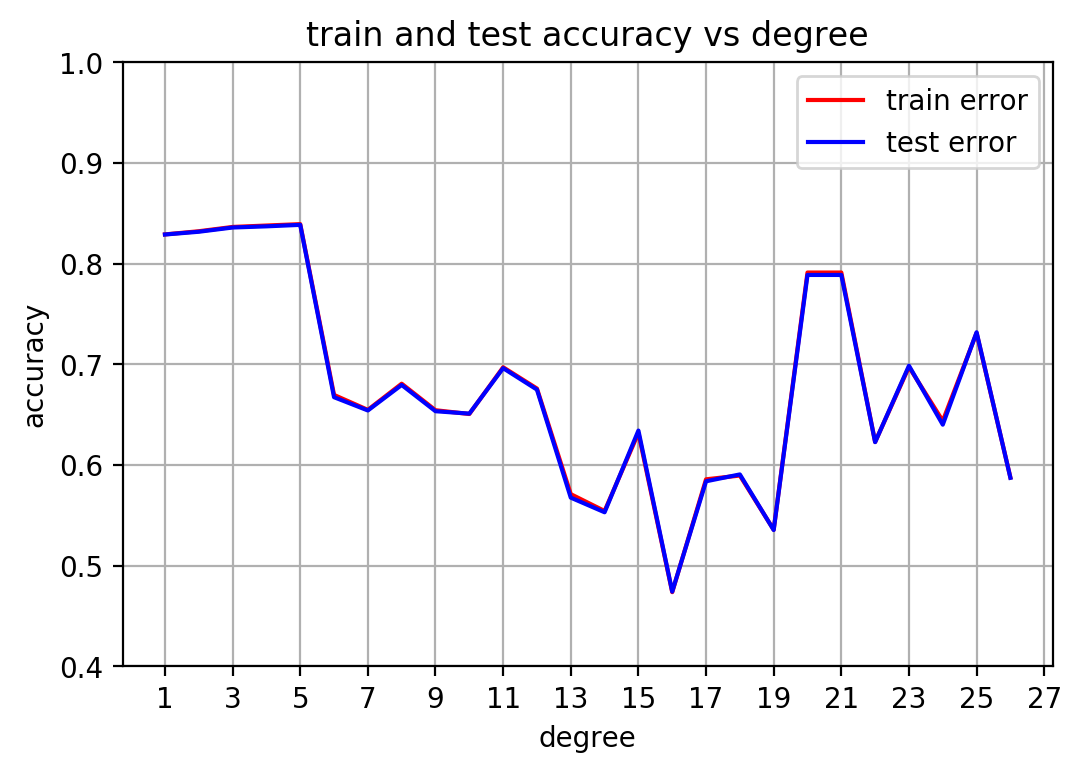
\includegraphics[width=8cm]{accuracy_vs_degree.png}
  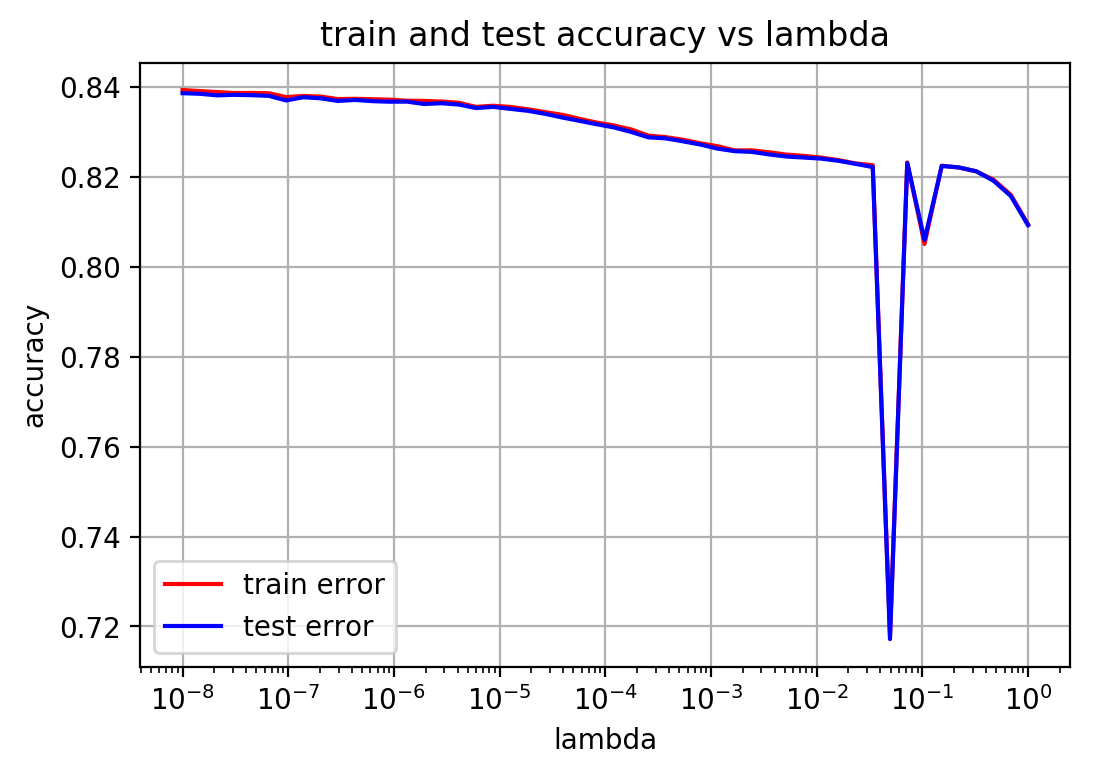
\includegraphics[width=8cm]{accuracy_vs_lambda.png}
  \caption{(Left) Training and testing accuracy for Ridge regression with jet=0, lambda=1e-8, for different degrees of polynomial expansion.}
  \label{fig:figure 1}
  \caption{(Right) Training and testing accuracy for Ridge regression with jet=0, degree=5, for different values of lambda.}
  \label{fig:figure 2}
\end{figure}

\mbox{}\\

\begin{table}[h!]
  \centering
  \begin{tabular}{|c|c|c|}
    \hline
    \textbf{Model} & \textbf{Testing accuracy} & \textbf{Variance}\\
    \hline
    Least squares & 0.844675385334 & 2.76e-07\\
    \hline
    Ridge regression & 0.844635350637 & 5.58e-07\\
    \hline
    Regularized logistic regression & 0.826116982945 & 1.3884e-05\\
    \hline
  \end{tabular}
  \caption{Accuracy and standard deviation for our models (for jet=0)}
  \label{tab:table 1}
\end{table}

\section{Conclusion}
As we can see in the table, least squares has the highest accuracy, but we selected the model with the best score on Kaggle, ridge regression. This certainly comes from the fact that least squares has no lambda hyper-parameter to penalize over fitting. Because of this, the local score wasn't always equivalent to the kaggle score.\\

It is worth saying that we tried a method which would determine which two columns we should add the product to the features in order to increase the score, but even after determining which columns product to add for each jet, the total accuracy was smaller.


\end{document}
